\documentclass[border=5pt]{standalone}
\usepackage{tikz}
\usepackage{tikz-3dplot}
\usetikzlibrary{arrows.meta, 3d, perspective, calc, matrix, positioning}
\usepackage{amsmath}
\begin{document}
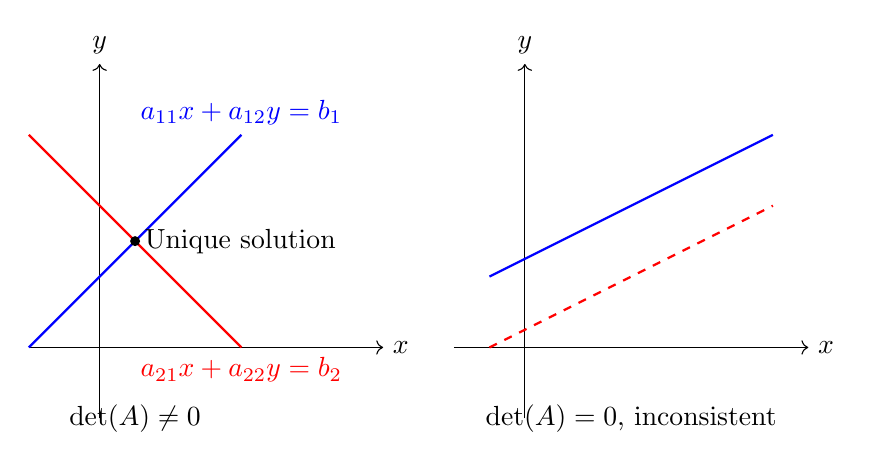
\begin{tikzpicture}[scale=0.9]
    % Coordinate axes
    \draw[->] (-1,0) -- (4,0) node[right] {$x$};
    \draw[->] (0,-1) -- (0,4) node[above] {$y$};

    % Unique solution case
    \begin{scope}[shift={(-0.5,0)}]
        \draw[thick, blue] (-0.5,0) -- (2.5,3) node[above] {$a_{11}x + a_{12}y = b_1$};
        \draw[thick, red] (-0.5,3) -- (2.5,0) node[below] {$a_{21}x + a_{22}y = b_2$};
        \fill (1,1.5) circle (2pt) node[right] {Unique solution};
        \node at (1,-1) {$\det(A) \neq 0$};
    \end{scope}

    % Parallel lines case
    \begin{scope}[shift={(6,0)}]
        \draw[->] (-1,0) -- (4,0) node[right] {$x$};
        \draw[->] (0,-1) -- (0,4) node[above] {$y$};

        \draw[thick, blue] (-0.5,1) -- (3.5,3);
        \draw[thick, red, dashed] (-0.5,0) -- (3.5,2);
        \node at (1.5,-1) {$\det(A) = 0$, inconsistent};
    \end{scope}
\end{tikzpicture}
\end{document}
